\documentclass{beamer}

\usepackage[T1]{fontenc}
\usepackage[utf8]{inputenc}
\usepackage{lmodern}
\usepackage{graphicx}
\usepackage{svg}

\usetheme{Warsaw}
\logo{
\includegraphics[height=1cm]{assets/dna.png}}

\title[A.C. en la Simulación de la Dinámica de Dominios Proteicos]{Autómatas Celulares en la Simulación de la Dinámica de Dominios Proteicos}
\author[Universidad Nacional Autónoma de México]{Juan C. Castrejón E.}
\institute{Universidad Nacional Autónoma de México}
\date{6 de Junio de 2023}

\begin{document}

\begin{frame}
\titlepage
\end{frame}

\begin{frame}{Tabla de Contenidos}
\tableofcontents
\end{frame}

\section{Introducción}

\begin{frame}{Importancia de la evolución de dominios de proteínas en la biología y medicina.}
\begin{itemize}
    \item Pueden proporcionar información sobre la historia de la vida y la función de los organismos actuales.
    \item Se podría prever cómo progresarían las enfermedades o cómo podrían evolucionar los patógenos, lo que puede informar el desarrollo de nuevos tratamientos o medicamentos.
\end{itemize}
\end{frame}

\begin{frame}{Uso de métodos computacionales para modelar y predecir la evolución de dominios de proteínas.}
\begin{itemize}
    \item Aprovechar el modelo de sustitución de aminoácidos propuesto por Margaret Dayhoff.
\end{itemize}
\begin{figure}[ht]
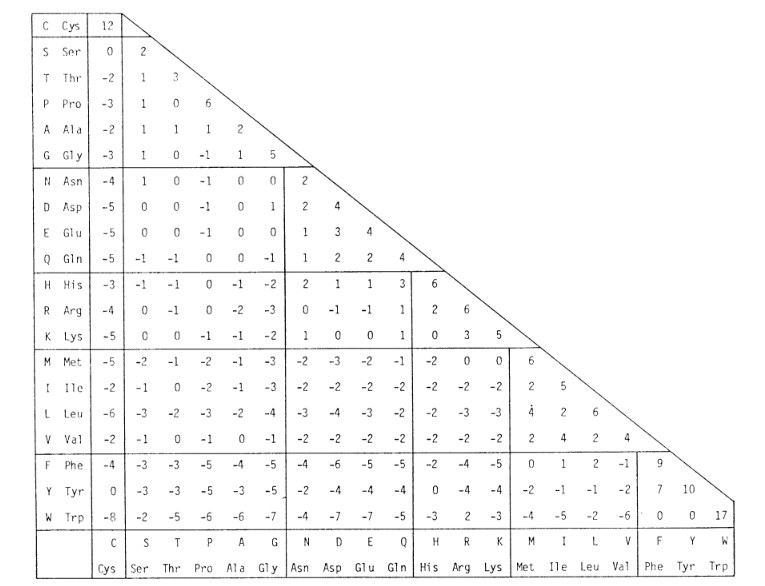
\includegraphics[width=0.45\textwidth]{assets/dayhoff.jpg}
\caption{Matriz de Dayhoff.}
\label{fig:dayhoff.svg}
\end{figure}
\end{frame}

\begin{frame}{Autómatas celulares como herramienta poderosa para modelar sistemas dinámicos complejos.}
\begin{itemize}
    \item Los autómatas celulares son modelos matemáticos que simulan sistemas complejos mediante reglas simples. Un autómata celular tiene una cuadrícula de celdas, cada una de las cuales puede estar en un número finito de estados. El estado de una celda en un momento dado depende de su propio estado y del estado de sus vecinos en el paso de tiempo anterior, según un conjunto de reglas de transición.
\end{itemize}
\end{frame}

\begin{frame}{Autómatas celulares como herramienta poderosa para modelar sistemas dinámicos complejos.}
\begin{figure}[ht]
\includesvg[width=0.35\textwidth]{assets/CA.svg}
\caption{Ejemplos de reglas.}
\label{fig:CA.svg}
\end{figure}
\end{frame}

\begin{frame}{Autómatas celulares como herramienta poderosa para modelar sistemas dinámicos complejos.}
\begin{figure}[ht]
\centering
\includesvg[width=0.42\textwidth]{assets/CA2.svg}
\caption{Ejemplos de reglas propagadas.}
\label{fig:CA2.svg}
\end{figure}
\end{frame}

\section{Pregunta de Investigación}
\begin{frame}{Pregunta de Investigación}
\begin{itemize}
\item ¿Cómo se pueden utilizar los autómatas celulares para simular la evolución de dominios de proteínas?
\end{itemize}
\end{frame}

\section{Objetivo}
\begin{frame}{Objetivo}
\begin{itemize}
\item Desarrollar un modelo basado en autómatas celulares para simular la evolución de dominios de proteínas.
\end{itemize}
\end{frame}

\section{Método}
\begin{frame}{Método}
\begin{itemize}
\item Crear un autómata celular para representar la estructura y función de una proteína.
\item Definir reglas de transición basadas en la dinámica de evolución de dominios de proteínas.
\item Simular la evolución de dominios de proteínas utilizando el autómata celular propuesto.
\end{itemize}
\end{frame}

\section{Definición del automáta}
\begin{frame}{Definición del automáta}
\begin{itemize}
    \item Se utilizará un autómata celular 1D (CA) para simular la evolución del dominio de las proteínas.
    \item El CA es un arreglo unidimensional de celdas, cada una con uno de (g+3) posibles estados, que representan clases de dominios, dos símbolos de terminación y un estado vacío.
    \item Al inicializar, la celda central se establece en un dominio ancestral, mientras que las demás se configuran como vacías.
    \item El CA evoluciona durante una cantidad de pasos de tiempo igual al número de dominios en la proteína con la mayor cantidad de dominios en el conjunto de datos de entrenamiento.
\end{itemize}
\end{frame}

\begin{frame}{Reglas de transición}
\begin{itemize}
    \item Regla A (Herencia): Si una celda ha evolucionado hacia un dominio (es decir, su estado no es "0/"), heredará este dominio en el próximo paso de tiempo.
    \item Regla B (Evolución de adelante hacia atrás): Si una celda y su vecino de la derecha están ambos en el estado vacío, y su vecino de la izquierda está en un estado de dominio, la celda evolucionará hacia un dominio en el próximo paso de tiempo. El dominio se selecciona utilizando el algoritmo de selección de ruleta basado en la matriz F2B (probabilidad previa de evolución de adelante hacia atrás).

\end{itemize}
\end{frame}

\begin{frame}{Reglas de transición}
\begin{itemize}
    \item Regla C (Evolución de atrás hacia adelante): Si una celda y su vecino de la izquierda están ambos en el estado vacío, y su vecino de la derecha está en un estado de dominio, la celda evolucionará hacia un dominio en el próximo paso de tiempo. El dominio se selecciona utilizando el algoritmo de selección de ruleta basado en la matriz B2F (probabilidad previa de evolución de atrás hacia adelante).

    \item Regla D (Retorno a la inanimación): Si una celda y sus vecinos están todos en el estado   vacío, la celda permanecerá en el estado vacío en el próximo paso de tiempo.
\end{itemize}
\end{frame}

\begin{frame}{Reglas de transición}
\begin{figure}[ht]
\centering
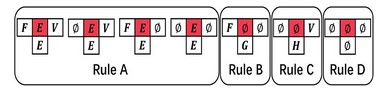
\includegraphics[width=0.5\textwidth]{assets/reglas.jpg}
\caption{Ayuda visual para reglas.}
\label{fig:reglas.jpg}
\end{figure}
\end{frame}

\section{Resultados}
\begin{frame}{Resultados}
\begin{itemize}
\item Se ha mostrado una implementación novedosa para representar la evolución de los dominios proteicos, tomando como ventaja la naturaleza compleja de los autómatas celulares para reflejar con simplicidad un fénomeno difícil de estudiar que se puede aprovechar en múltiples áreas científicas.
\end{itemize}
\end{frame}

\section{Futuro}
\begin{frame}{Futuro}
\begin{itemize}
\item La implementación usa dominios proteicos tomados de una base de datos establecida para generar estructuras reales.
\item Un proceso llamado MDAT (herramiento de alineacion multi dominio) puede ser usada con estructuras reales y las generadas por este método para producir valores útiles que miden la similitud en la evolución de las proteinas.
\item ¿Qué tan factibles son los métodos de generación aleatoria para la búsqueda de estructuras?
\end{itemize}
\end{frame}


\begin{frame}{Referencias}
\begin{itemize}
    \item Qiu, Y., Zhang, X. (2020). Using Cellular Automata to Simulate Domain Evolution in Proteins. Frontiers in Genetics, 11, 515. \url{https://doi.org/10.3389/fgene.2020.00515}
    \item Schwartz, J. T., Neumann, J. V., and Burks, A. W. (1967). Theory of self-reproducing automata. Q. Rev. Biol. 21:745. doi: 10.2307/2005041
    \item Dayhoff, M.O., Schwartz, R.M. and Orcutt, B.C. (1978) A model of evolutionary change in proteins, in Dayhoff, M.O. Edition, Atlas of Protein Sequence and Structure. Natl. Biomed. Res. Found., Washington DC, 5(3), 345- 352.
\end{itemize}
\end{frame}

\begin{frame}{Recursos}
\begin{itemize}
\item Repositorio de Github \url{https://github.com/JCastrejonE/proyecto-computacion-genomica/tree/main/}
\item Código de esta presentación \url{https://github.com/JCastrejonE/proyecto-computacion-genomica/blob/main/presentacion/main.tex}
\end{itemize}
\end{frame}

\end{document}